\let\negmedspace\undefined
\let\negthickspace\undefined
\documentclass[journal]{IEEEtran}
\usepackage[a5paper, margin=10mm, onecolumn]{geometry}
%\usepackage{lmodern} % Ensure lmodern is loaded for pdflatex
\usepackage{tfrupee} % Include tfrupee package

\setlength{\headheight}{1cm} % Set the height of the header box
\setlength{\headsep}{0mm}     % Set the distance between the header box and the top of the text

\usepackage{gvv-book}
\usepackage{gvv}
\usepackage{cite}
\usepackage{amsmath,amssymb,amsfonts,amsthm}
\usepackage{algorithmic}
\usepackage{graphicx}
\usepackage{textcomp}
\usepackage{xcolor}
\usepackage{txfonts}
\usepackage{listings}
\usepackage{enumitem}
\usepackage{mathtools}
\usepackage{gensymb}
\usepackage{comment}
\usepackage[breaklinks=true]{hyperref}
\usepackage{tkz-euclide} 
\usepackage{listings}
% \usepackage{gvv}                                        
\def\inputGnumericTable{}                                 
\usepackage[latin1]{inputenc}                                
\usepackage{color}                                            
\usepackage{array}                                            
\usepackage{longtable}                                       
\usepackage{calc}                                             
\usepackage{multirow}                                         
\usepackage{hhline}                                           
\usepackage{ifthen}                                           
\usepackage{lscape}
\usepackage{circuitikz}
\tikzstyle{block} = [rectangle, draw, fill=blue!20, 
    text width=4em, text centered, rounded corners, minimum height=3em]
\tikzstyle{sum} = [draw, fill=blue!10, circle, minimum size=1cm, node distance=1.5cm]
\tikzstyle{input} = [coordinate]
\tikzstyle{output} = [coordinate]


\begin{document}

\bibliographystyle{IEEEtran}
\vspace{3cm}

\title{8-8.3-3}
\author{EE24BTECH11064 - Harshil Rathan}
 \maketitle
% \newpage
% \bigskip
{\let\newpage\relax\maketitle}

\renewcommand{\thefigure}{\theenumi}
\renewcommand{\thetable}{\theenumi}
\setlength{\intextsep}{10pt} % Space between text and floats


\numberwithin{equation}{enumi}
\numberwithin{figure}{enumi}
\renewcommand{\thetable}{\theenumi}

\textbf{Question}:\\
Find the area of the region lying in the first quadrant and bounded by $y=4x^2$, $x=0$, $y=1$ and $y=4$. \\ 
\solution \\
THe equation of the curve is 
\begin{align}
     y = 4x^2
     \label{0.1}
\end{align}
\begin{align}
    x = \frac{\sqrt{y}}{2}
\end{align}
w.k.t that \ref{0.1} is an upward parabola symmetric about y-axis\\
\textbf{Point of intersection}\\
Expressing the equation of parabola in matrix form $g\brak{\vec{x}}= \vec{x}^{\top}\vec{V}\vec{x}+2\vec{u}^{\top}\vec{x}+f=0$,
\begin{align}
  \myvec{x&y}\myvec{4&0\\0&0}\myvec{x\\y}+2\myvec{0 & -\frac{1}{2}}\myvec{x\\y}+0=0
\end{align}
The general form of a line equation can be expressed as
\begin{align}
    \vec{m}^\top \vec{x} = c
\end{align}
For $y=1$
\begin{align}
    \vec{m} = \begin{pmatrix} 0 \\ 1 \end{pmatrix}, \quad c = 1
\end{align}
For $y=4$
\begin{align}
    \vec{m} = \begin{pmatrix} 0 \\ 1 \end{pmatrix}, \quad c = 4
\end{align}
Intersection of a line and a conic is given by,
\begin{align}
  \kappa_i=\frac{-\vec{m}^{\top}\brak{\vec{Vh}+\vec{u}}\pm\sqrt{\sbrak{\vec{m}^{\top}\brak{\vec{Vh}+\vec{u}}}^2-g\brak{h}\brak{\vec{m}^{\top}\vec{Vm}}}}{\vec{m}^{\top}\vec{Vm}}
\end{align}
On substituting and solving \\
The intersection points in the first quadrant are 
\begin{align}
    \left( \frac{1}{2}, 1 \right),  (1, 4)
\end{align}
\textbf{Theory} \\ 
There are two ways to solve the above integral, Theoretically and Computationally (trapezoid method). We shall compare the results obtained by both methods.
\begin{align}
    \int_1^4 x \, dx = \int_1^4 \left| \frac{\sqrt{y}}{2} \right| dy
\end{align}
\begin{align}
    \frac{1}{2} \int_1^4 y^{\frac{1}{2}} \, dy = \frac{1}{2} \left| \frac{y^{\frac{3}{2}}}{\frac{3}{2}} \right|_1^4
\end{align}
\begin{align}
    = \frac{1}{2} \cdot \frac{2}{3} \left[ 4^{\frac{3}{2}} - 1^{\frac{3}{2}} \right]
\end{align}
\begin{align}
    = \frac{1}{3} \left( 4\sqrt{4} - 1 \right) = \frac{1}{3} (8 - 1) = \frac{7}{3} \ = 2.3333 \text{ sq. units.} 
\end{align}
\textbf{Solution using Trapezoidal Rule}\\
Taking trapezoid shaped strips of small area and adding them all up. Say we have to find the area of $y_{x}$ from $x=x_0$ to $x=x_n$, discretize points on the $x$ axis $x_0, x_1, x_2, \dots, x_n$ such that they are equally spaced with step-size $h$. \newline
To apply the trapezoidal rule, we discretize the \( x \)-axis into \( n \) equally spaced intervals, with \( h = \frac{1}{n} \). The points on the \( x \)-axis are \( x_0, x_1, x_2, \dots, x_n \), where:

\begin{align}
x_0 = 0, \quad x_1 = h, \quad x_2 = 2h, \dots, \quad x_n = 1    
\end{align}

Sum of all trapezoidal areas is given by
\begin{align}
  A&=\frac{1}{2}h\brak{y\brak{x_1}+y\brak{x_0}}+ \frac{1}{2}h\brak{y\brak{x_2}+y\brak{x_1}}+\dots+\frac{1}{2}h\brak{y\brak{x_n}+y\brak{x_{n-1}}}\\
  &=h\sbrak{\frac{1}{2}\brak{y\brak{x_0}+y\brak{x_n}}+ y\brak{x_1}+\dots+y\brak{x_{n-1}}}
\end{align}
Substituting \( y(x_n) = 4x_n^2 \), we get:

\begin{align}
    A = h \left( \frac{1}{2} \left( 4x_0^2 + 4x_n^2 \right) + \sum_{i=1}^{n-1} 4x_i^2 \right)
\end{align}
Since \( x_0 = 0 \) and \( y(x_0) = 0 \), this simplifies to:

\begin{align}
    A = h \left( \frac{1}{2} \left( 4x_n^2 \right) + \sum_{i=1}^{n-1} 4x_i^2 \right)
\end{align}
Let $A\brak{x_n}$ be the area enclosed by the curve $y\brak{x}$ from $x=x_0$ to $x=x_n$, $\brak{x_0, x_1, \dots x_n}$ be equidistant points with step-size $h$.
\begin{align}
  A\brak{x_n+h}=A\brak{x_n}+\frac{1}{2}h\brak{y\brak{x_n+h}+y\brak{x_n}}
\end{align}
Discretizing the steps, making $A\brak{x_n}=A_n, y\brak{x_n}=y_n$ we get,
\begin{align}
 A_{n+1}=A_n+\frac{1}{2}h\brak{y_{n+1}+y_n}
\end{align}
\begin{align}
    A_{n+1} = A_n + \frac{1}{2} h \left( 4x_{n+1}^2 + 4x_n^2 \right)
\end{align}
So the final simplified formula is
\begin{align}
    A_{n+1} = A_n + 2h \cdot \left( x_{n+1}^2 + x_n^2 \right)
\end{align}
The solution is hence verified with the theoretical solution
\\
Area required is $2.3333$ sq.units
\begin{figure}
    \centering
    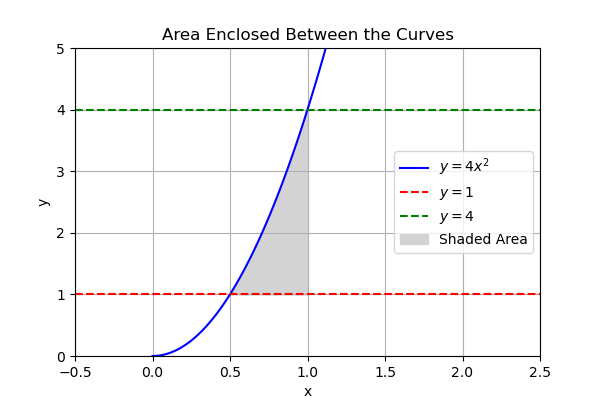
\includegraphics[width=\columnwidth]{figs/Figure_1.png}
\end{figure}
\end{document}



